\section{Entity Ranking}
\label{sec:ranking}

In this section, we first introduce a model for the Web of Data and define what is an entity, i.e., the unit of information that is queried and retrieved. Then we explain how to adapt two field-based ranking frameworks, i.e., the Probabilistic Relevance Framework~\cite{Robertson:2009:PRF} and the Divergence From Randomness~\cite{amati:2002:acm}, to this model.

\subsection{The Web of Data}
\label{sec:wod}

We define the \emph{Web of Data} as the collection of structured data sources that are exposed on the Web through a wide range of forms such as HTML tables, Deep Web databases, XML documents, documents embedding semantic markups, e.g., Microformats, Microdata, RDF, RDFa. Since each data source might have its own defined schema, ranging from loosely to strictly defined, the data structure does not follow strict rules as in a database. Even within a given data source, the schema might not be fixed and may change as the information grows. The information structure evolves over time and new entities can require new attributes. We therefore consider the Web of Data as being \emph{semi-structured}~\cite{abiteboul:1997:icdt}.

\paragraph{Web of Data Model} In the rest of this paper, we assume that a common graph-based data model, based on the Resource Description Framework (RDF) model~\cite{klyne_carroll:2004}, is used for all the semi-structured data sources based on the Web. RDF is a generic data model that can be used for inter-operable data exchange. A resource, i.e., an entity, is described in such a way that it can be processed by machines automatically. In RDF, a resource description is composed of statements about the resource. A statement is a triple consisting of a subject, a predicate and an object, and asserts that a subject has a property with some object. A set of RDF statements forms a directed labelled graph. In an RDF graph, as displayed in Figure~\ref{fig:rdf-graph}, a node can be of three types: URI, literal and blank node. A URI serves as a globally-unique identifier for a resource. A literal is a character string with an optional associated language and datatype. A blank node represents a resource for which a URI is not given.

\paragraph{Entity Extraction} There are multiple ways to extract entities from an RDF graph. Here, we use the approach described in~\cite{delbru:jws:entity}, where we consider an entity as a star graph, i.e., a subgraph with a central node and its direct neighbor nodes it links to. Figure~\ref{fig:rdf-graph} displays how the RDF graph can be split into four entities \emph{me}, \emph{\_:b1}, \emph{\_:b2} and \emph{paper/547}. Each entity description forms a subgraph containing the incoming and outgoing edges of the entity node. In order to simplify the extraction process, we only consider the outgoing edges of a star graph.
% Our entity extraction process and representation are similar in nature to the ``Hierarchical Entity Model proposed'' in~\cite{neumayer:2012:ecir}.

\paragraph{Entity Model} In the remainder of the paper, the unit of information which is retrieved and ranked is an \emph{entity}~\cite{delbru:jws:entity} and is formalised as a list of attribute-value pairs:
\begin{description}[noitemsep,nolistsep]
  \item[Entity] represents a set of attribute-value pairs and is identified by the entity node label, e.g., \emph{paper/547};
  \item[Attribute] is an edge linking the entity node to one of its neighbor nodes and is identified by the edge label, e.g., \emph{title}, \emph{name} or \emph{creator};
  \item[Value] is a neighbor node of the entity node and is identified by the node label, e.g., \emph{Object-} or \emph{paper/547}. A value is always associated to one attribute. Multiple values can be associated to a same attribute, such as the nodes \emph{\_:b1} and \emph{\_:b2} with the attribute \emph{knows} of the entity \emph{me}.
\end{description}

\begin{figure}
\centering
\resizebox{0.65\textwidth}{!}{
    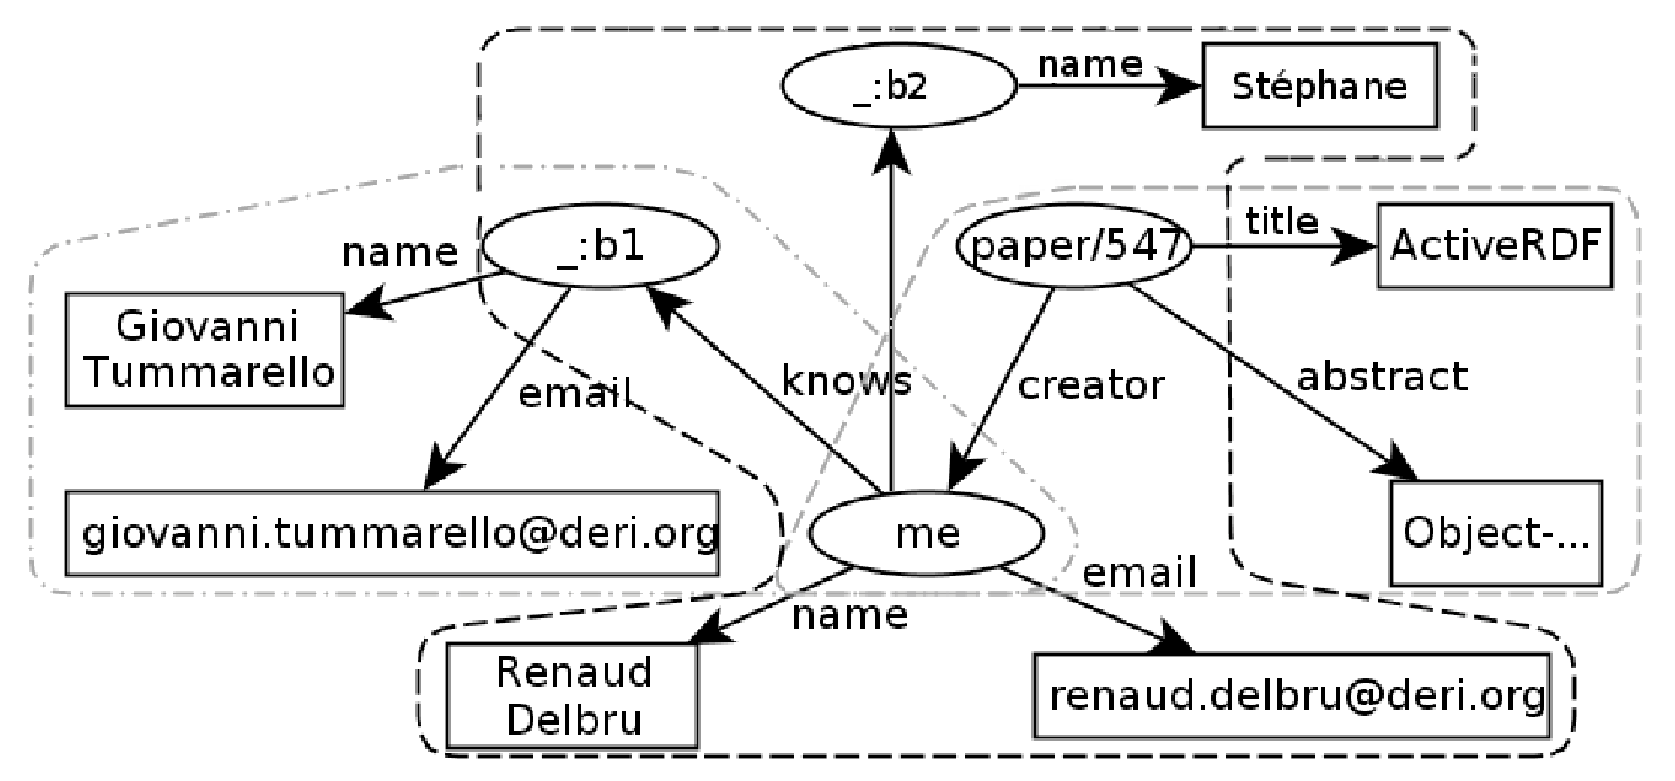
\includegraphics[scale=1]{figures/rdf-graph}
}
\caption{An RDF graph divided into four entities identified by the nodes \emph{me}, \emph{\_:b1}, \emph{\_:b2} and \emph{paper/547}.}
\label{fig:rdf-graph}
\vspace{-1em}
\end{figure}

%\subsection{Ranking in the Web of Data}
\subsection{Field-Based Ranking Models}
\label{sec:ranking-wod}

In this section, we explain how to adapt two existing field-based ranking frameworks to the entity model. In the Probabilistic Relevance Framework (PRF), BM25F~\cite{zaragoza:2004:microsoft} is a popular web-search ranking function for field-based document retrieval where a document is composed of multiple normalized weighted fields. For example, a field can be the title, the author or the body of the document. The Divergence From Randomness (DFR) framework gives birth to many ranking models, in particular  PL2F~\cite{macdonald:2005:clef} which considers field-based documents similarly to BM25F. The mapping from the field-based document model to the entity model is straightforward. An entity can be seen as a document and an entity attribute as a document field. In presence of a multi-valued attribute, the common approach is to merge the content of all the values into one single value, i.e., creating a single bag of words.% However, this simplification of the underlying data model is inadequate for structured data. Therefore, we propose an extension of field (i.e., attribute) based ranking model in Section~\ref{sec:mf-model} to deal with multi-valued attributes.

\paragraph{Ranking Features}

The following features are used in the field-based ranking functions:
\begin{description}[noitemsep,nolistsep]
  \item[field length] refers to the number of terms in a value node label. In case of a multi-valued attribute, it refers to the number of terms across all the values associated to the attribute.
  \item[average field length] is equal to the mean of \emph{field length} across entities.
\end{description}

\paragraph{BM25F Ranking Function}

Using BM25F, an entity $e$ is scored with regard to a query $q$ as follows:
\begin{eqnarray}
  Score(e,q) & = & \alpha_e\times\sum_{t\in q}{q_t\times tfn_e \times \omega_t}\\
  \label{eq:tfidf-score}
  tfn_e & = & \frac{f_{t,e}\times(k_1+1)}{f_{t,e}+k_1} \\
  \label{eq:bm25f_2}
  f_{t,e} & = &
  \sum_{a\in e}{\frac{\alpha_a\times f_{t,e,a}}{1+b_a\times\left(\frac{l_{e,a}}{l_a}-1\right)}}
  \label{eq:bm25f_1}
\end{eqnarray}
where $q_t$ is the weight of the query $q$ for the term $t$, i.e., its frequency within the query $q$, $tfn_e$ is the term frequency normalisation function, $\omega_t$ is the Inverse Document Frequency (IDF) function of the term $t$, $k_1$ is the saturation parameter, $f_{t,e,a}$ is the frequency of the term $t$ in the attribute $a$ of the entity $e$, $\alpha_a$ is a weight of the attribute $a$ and $\alpha_e$ a weight of the entity $e$, $b_a$ is the normalisation parameter for the attribute $a$ with $b_a \in \left[0,1\right]$, $l_{e,a}$ is the \emph{field length} of the attribute $a$ in the entity $e$, $l_a$ is the \emph{average field length} of the attribute $a$. The IDF is defined as
$
\omega_t=1+log\left(\frac{N}{v_t+1}\right)
$,
where $N$ is the total number of entities in the collection and $v_t$ is the total number of entities that have occurrences of the term $t$.

\paragraph{PL2F Ranking Function}

DFR weighting models are based on the combination of three components, i.e., the information gain, the randomness model and the term frequency normalisation model. PL2F bases the information gain on the Laplace after-effect model, uses Poisson as the model for randomness, and the \emph{normalisation 2F} for the term frequency normalisation.
Using PL2F, an entity $e$ is scored with regard to a query $q$ as follows:
\begin{eqnarray*}
  Score(e,q) & = & \alpha_e\times\sum_{t\in q}{qtw \times w_{e,t}}\\
  \label{eq:dfr-score}
  w_{e,t} & = & \left(1-P_{risk}\right) \times \left(-log_2\left(P_{P}\right)\right) \\
  \label{eq:dfr-term-weight}
  P_{risk} & = & \frac{tfn_e}{1+tfn} \\
  \label{eq:dfr-prisk}
  P_{P} & = & \frac{\lambda^{tfn_e}}{tfn!}\times e^{-\lambda} \:\text{ where }\: \lambda=\frac{TF}{N} \\
  \label{eq:dfr:rand-poisson}
\end{eqnarray*}
where $qtw=\frac{q_t}{q_{t,max}}$ is the weight of the query $q$ for the term $t$ with $q_{t,max}$ the maximum of $q_t$ in $q$, $w_{e,t}$ is the weight of the term $t$ in the entity $e$, $1-P_{risk}$ estimates the information gain of a term $t$, $-log_2\left(P_{P}\right)$ evaluates the importance of a term $t$ in the entity $e$ thanks to the Poisson model and $TF$ is equal to the frequency of the term $t$ in the collection. The factorial is approximated with the Stirling's formula \mbox{$tfn_e!=\sqrt{2\pi}\times tfn^{tfn+0.5}\times e^{-tfn}$}.
The term frequency of the term $t$ in the entity $e$ is normalized as follows:
\begin{equation}
  tfn_e = \sum_{a\in e}{\alpha_a\times f_{t,e,a} \times log_2\left(1+c_a\times\frac{l_a}{l_{e,a}}\right)}
  \label{eq:pl2f}
\end{equation}
where $c_a$ is a per-attribute hyperparameter with $c_a \in\;]0,+\infty[$.
